\graphicspath{{figs/3a}}
\chapter{Bayesian Linear Regression}


%   ┌──────────────────────────────────────────────────────────────────────────┐
%   │ Summary                                                                  │
%   └──────────────────────────────────────────────────────────────────────────┘


\section{Linear Basis function model}
\subsection{Gaussian basis functions}
\paragraph*{1.2. Recall closed form of the posterior distribution in linear case. Then, code and visualize posterior sampling. What can you observe?}

Let $N$ denote the number of training examples, $K$ the number of dimensions of the outputs, and $p$ the number of features (or predictors) in the input data. Consider $X \in \mathbb{R}^{N \times p}$, the input matrix, and $Y \in \mathbb{R}^{N \times K}$, the output matrix. 

We typically define the posterior distribution as $ p(w | X, Y) $. This distribution represents our updated beliefs about the parameters $ w $ after observing the data $ X $ and $ Y $. According to Bayes' rule, we can express the posterior distribution as the product of two components:
\begin{enumerate}
    \item $ p(w) $, which represents our prior beliefs about the distribution of $ w $ before observing the data.
    \item $ p(Y | X, w) $, indicating the probability of observing the data $ Y $ given the parameters $ w $ and the data $ X $. This quantifies how likely our data is under different hypotheses represented by $ w $.
\end{enumerate}
Therefore, the formula for the posterior distribution is given by:
\[ p(w | X, Y) \propto p(Y | X, w) p(w) \]

In this formula, we start with our initial beliefs (priors) and then update these beliefs based on the new data (likelihood). In the case of our linear model, we know that $ y_i = \Phi^T_i w + \epsilon $, with $ \Phi \in \mathbb{R}^{N \times (p + 1)} $ representing the design matrix and $ \epsilon $ denoting the residual. Assuming that the error follows a centered Gaussian distribution with standard deviation $ \beta ^{-1} = 2\sigma^2 $, meaning that $ \epsilon \sim \mathcal{N}(0, \beta ^{-1}) $. Consequently, we can conclude that:
\[ p(y_i | x_i, w) \sim \mathcal{N}(\Phi^T_i w, \beta ^{-1}) \]

Furthermore, we selected a centered Gaussian prior with a variance of $ \alpha^{-1}I $ where $\alpha$ governs the prior distribution over the weights $\mathbf{w}$:
\[ p(w | \alpha) \sim \mathcal{N}(0, \alpha^{-1}I) \]

In this specific case, we can demonstrate that the posterior distribution $ p(w | X, Y) $ follows a Gaussian distribution as follows:
\[ p(w | X, Y) \sim \mathcal{N}(\boldsymbol{\mu}, \boldsymbol{\Sigma}) \]

The precision matrix $ \boldsymbol{\Sigma} $, which is the inverse of the covariance matrix of the distribution parameters, is defined as:
\[ \boldsymbol{\Sigma}^{-1} = \alpha I + \beta \Phi^T \Phi \]

The mean of the distribution parameters is given by:
\[ \boldsymbol{\mu} = \beta \boldsymbol{\Sigma} \Phi^T Y \]

Parameters $\alpha$ and $\beta$ serve analogous roles, with $\alpha$ governing the prior distribution and $\beta$ regulating the likelihood.

Now, we can proceed to sample from the updated (with data) posterior distribution $p(w | X, Y)$. This process is demonstrated in \Cref{fig:posterior}, with $\alpha = 2$ and $\beta = (2 \times 0.2^2)^{-1}$. It is worth noting that when $N=0$, the posterior distribution $p(w|X,Y)$ simplifies to the prior distribution $p(w)$. As we increase the number of data points, we can observe how the model's certainty increase, demonstrated by the reduction in the variance of the parameters of the distribution. In other words, having more data points reduces aleatoric uncertainty.

\begin{figure}[H]
    \centering
    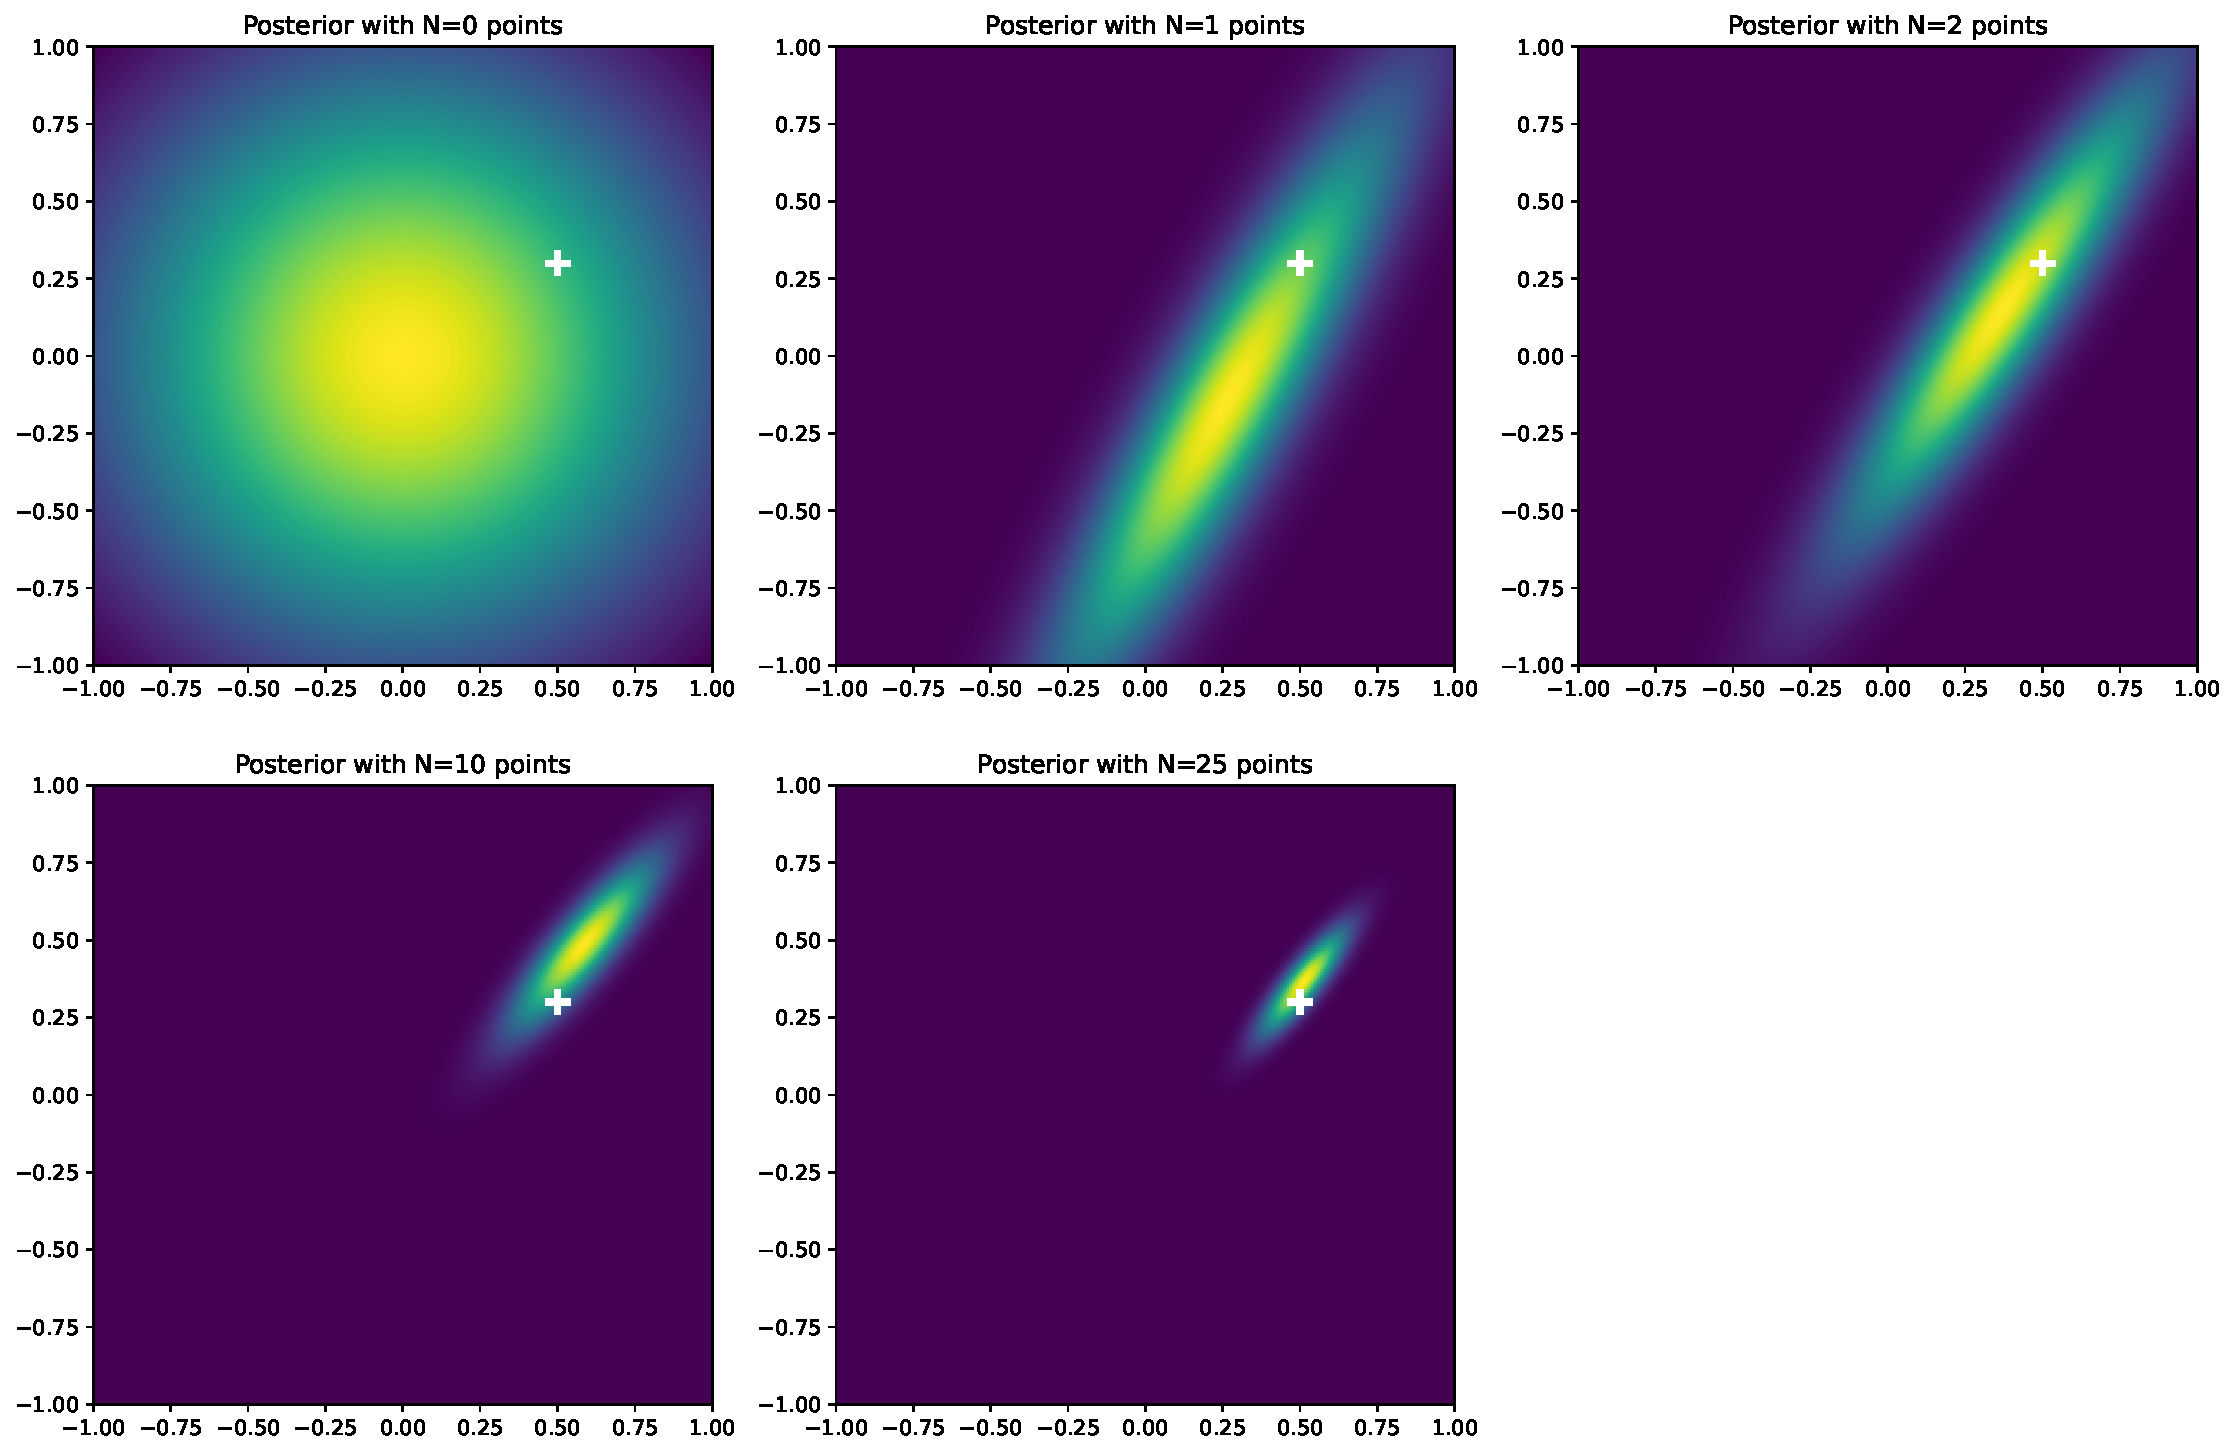
\includegraphics[width=0.95\textwidth]{posterior.pdf}
    \caption{Evolution of a Bayesian posterior distribution with increasing data points: A visual representation of Bayesian inference, depicting how the posterior distribution updates as more data is incorporated. From left to right, the figures show the posterior with $N=0$ (prior distribution), $N=1$, $N=2$, $N=10$, and $N=25$ data points, respectively. The cross mark represents the ground truth.}
    \label{fig:posterior}
\end{figure}

\paragraph*{1.3. Recall and code closed form of the predictive distribution in linear case.}
Using the information from the previous question, we can now calculate the predictive distribution for new data point $x^\star$ by marginalizing over the parameter $w$. This is represented by the following equation where $\mathcal{D} = \{X,Y\}$ denotes the dataset:
\[ p(y|x^\star , \mathcal{D}, \alpha, \beta ) = \int p(y| x^\star, w, \beta)p(w| \mathcal{D}, \alpha, \beta ) \]

By leveraging the property that the convolution of two Gaussian distributions results in another Gaussian distribution, we can demonstrate that the closed-form expression for the predictive distribution in the linear case is as follows:
\[ p\left(y|x^\star; \mathcal{D}, \alpha, \beta\right) = \mathcal{N}\left(y; \mu^T \boldsymbol{\Phi}(x^\star), \frac{1}{\beta} + \boldsymbol{\Phi}(x^\star)^T \boldsymbol{\Sigma} \boldsymbol{\Phi}(x^\star)\right) \]

We can see that the variance in the predictive distribution $ \sigma ^2_{pred} $  for a new observation can be divided into two parts:
\begin{enumerate}
    \item The aleatoric uncertainty, which represents the inherent noise in the data, that we fixed around $ \beta ^{-1}$;
    \item The epistemic uncertainty related to the model parameters $ w $, characterized by $\boldsymbol{\Phi}(x^\star)^T \boldsymbol{\Sigma} \boldsymbol{\Phi}(x^\star).$
\end{enumerate}
It's worth noting that as the number of data points $N$ approaches infinity ($ \lim_{N \to \infty} \boldsymbol{\Phi}(x^\star)^T \boldsymbol{\Sigma} \boldsymbol{\Phi}(x^\star) = 0 $), our understanding of the model parameters becomes nearly perfect. In this scenario, the only remaining source of uncertainty is the aleatoric uncertainty, stemming from the noise in the data.

\paragraph*{1.4. Based on previously defined \texttt{f\_pred()}, predict on the test dataset. Then visualize results using \texttt{plot\_results()} defined at the beginning of the notebook.}
\Cref{fig:phi_linear} illustrates a comparison between the predictions made by a Bayesian Linear Regression (BLR) model and the actual ground truth. In the left panel, you can see the model's linear fit to the training data, shown as blue points, alongside the true ground truth represented by the green line. To visualize the model's predictive uncertainty, shaded areas are used, ranging from dark to light, which correspond to one, two, and three standard deviation intervals, respectively.

The right panel of the figure focuses on the predictive variance \( \sigma ^2_{pred}  \) along the x-axis. This variance is depicted by a curve that widens as it moves away from the center of the training data, marked by the vertical dashed line. These visual elements together provide a comprehensive view of the model's confidence in its predictions across the entire domain.
\begin{figure}[H]
    \centering
    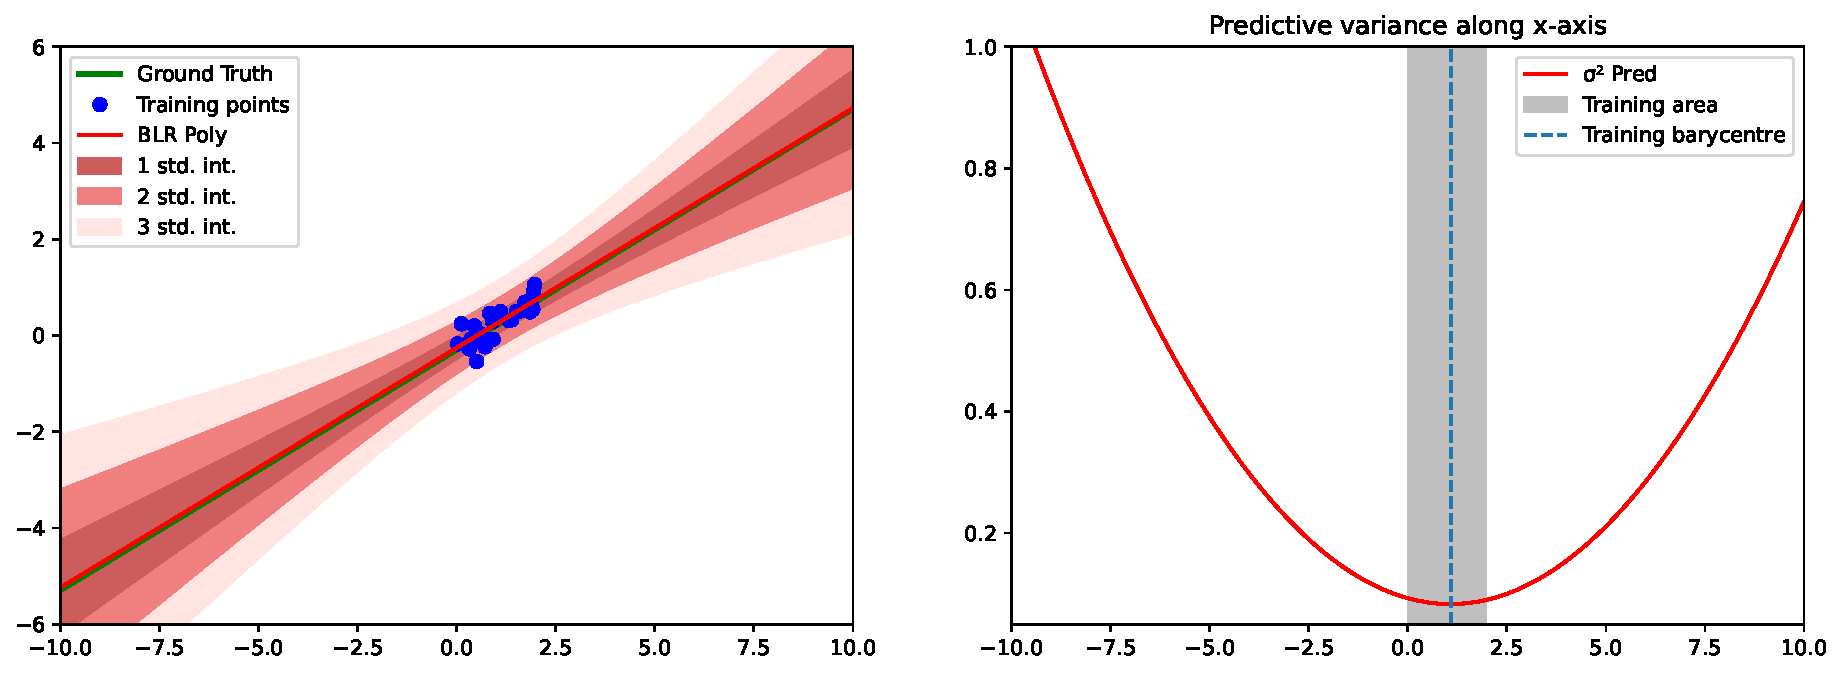
\includegraphics[width=0.95\textwidth]{phi_linear.pdf}
    \caption{The left panel illustrates the Bayesian Linear Regression (BLR) linear fit to the training data (blue points) against the ground truth (green line). The shaded areas represent the predictive uncertainty, with one, two, and three standard deviation intervals shown in progressively lighter shades. The right panel displays the predictive variance $\sigma ^2_{pred} $ across the x-axis. The vertical dashed line indicates the center of the training data.}
    \label{fig:phi_linear}
\end{figure}

\paragraph*{1.5. Analyse these results. Why predictive variance increases far from training distribution? Prove it analytically in the case where $\alpha=0$ and $\beta=1$.}

In the left panel of \Cref{fig:phi_linear}, we can observe that the confidence intervals are narrowest near the cluster of training points. This suggests higher confidence in predictions within this area. As we move away from the center of the training data (towards the extremities of the x-axis), the confidence intervals become wider, indicating increasing uncertainty in the model's predictions.

Looking at the right panel of \Cref{fig:phi_linear}, we notice that the variance remains low in the region where the training data is located (the grey shaded area). This correlates with the tight confidence intervals shown in the left panel. As expected, the predictive variance is lowest near the training barycentre, reflecting greater model certainty in this region due to the presence of more training data points.

As we move away from the training area on either side, the predictive variance increases significantly, which is consistent with the expanding confidence intervals in the left panel. This sharp increase in variance indicates a significant decrease in the model's confidence in its predictions outside the range of the training data. This is a common pattern in regression analysis, as the model has less data to rely on for predictions in these regions. Thus, the Bayesian Linear Regression model offers more reliable predictions within the training data range, with confidence diminishing as predictions move away from this range.\newline

\noindent Let's prove it analytically. With $\alpha = 0$ and $\beta = 1$, the computation of $\boldsymbol{\Sigma}^{-1}$ simplifies as follows:
\begin{align*}
    \boldsymbol{\Sigma}^{-1} 
        &= 0 \cdot I_3 + 1 \cdot \Phi^T \Phi \\
        &= \Phi^T \Phi \\ 
        &= \begin{pmatrix}
            1 & \dots & 1 \\
            x_1 & \dots & x_N
        \end{pmatrix} 
        \begin{pmatrix}
            1 & x_1 \\
            \vdots & \vdots \\
            1 & x_N 
        \end{pmatrix} \\
        &= \begin{pmatrix}
            N & \sum x_i \\
            \sum x_i & \sum x_i^2
        \end{pmatrix}
\end{align*}
To invert $\boldsymbol{\Sigma}$, we use the classic formula for a $2 \times 2$ matrix:
\[
    \boldsymbol{\Sigma} = \frac{1}{\det \boldsymbol{\Sigma}^{-1}} \begin{pmatrix}
        \sum x_i^2 & - \sum x_i \\
        - \sum x_i & N
    \end{pmatrix}
\]
Returning to our expression for $ \sigma^2_{pred} = \Phi (x^\star ) ^T \boldsymbol{\Sigma} \Phi (x^\star )$, we have:
\begin{align*}
    \sigma^2_{pred} = \Phi (x^\star ) ^T \boldsymbol{\Sigma} \Phi (x^\star ) &= \frac{1}{\det \boldsymbol{\Sigma}^{-1}} \begin{pmatrix}
        1 \\
        x^\star 
    \end{pmatrix} \begin{pmatrix}
        \sum x_i^2 & - \sum x_i \\
        - \sum x_i & N
    \end{pmatrix}\begin{pmatrix}
        1 & x^\star 
    \end{pmatrix} \\
    &= \frac{1}{\det \boldsymbol{\Sigma}^{-1}} \begin{pmatrix}1 \\ x^\star \end{pmatrix} \begin{pmatrix}\sum_i x_i^2 - x^\star \sum_i x_i & x^\star N - \sum_i x_i\end{pmatrix} \\
    &= \frac{1}{\det \boldsymbol{\Sigma}^{-1}}\left(\sum_i x_i^2 - x^\star \sum_i x_i + {x^\star }^2 N - x^\star \sum_i x_i\right) \\
    &= \frac{1}{\det \boldsymbol{\Sigma}^{-1}}\left(\sum_i x_i^2 - 2 x^\star \sum_i x_i + {x^\star }^2 N\right) \\
    &= \frac{1}{\det \boldsymbol{\Sigma}^{-1}}\sum_i \left(x_i - x^\star \right)^2
\end{align*}
This formula reveals that the predictive variance is directly proportional to the squared differences between each training data point $x_i$ and the prediction point $x^\star$. As $x^\star$ moves away from the region where the training data is concentrated, these squared differences increase, consequently leading to an increase in the predictive variance.

\paragraph*{Bonus: What happens when applying Bayesian Linear Regression on the following dataset?}

Looking at the right panel in \Cref{fig:phi_linear_hole}, we observe that the variance is surprisingly minized at the barycentre, i.e. the ''hole'' where there are not training data points. Typically, one would expect the variance to increase in regions with no data. This behavior suggests that the model is overconfident about its predictions in the gap, and we affirm this by observing low variance at the extremities.

\begin{figure}[H]
    \centering
    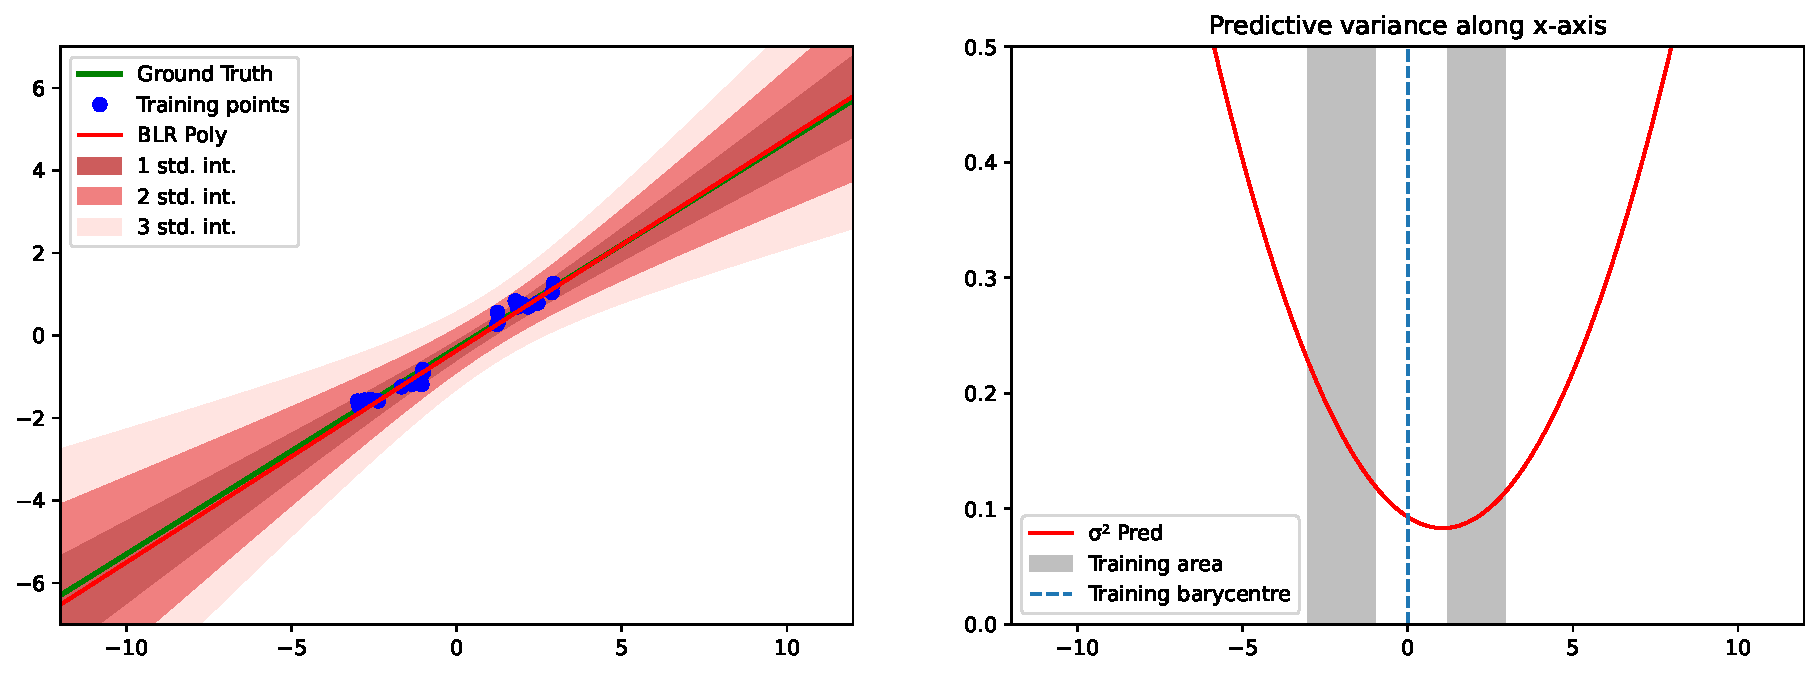
\includegraphics[width=0.95\textwidth]{phi_linear_hole.pdf}
    \caption{Visualization of predictive distribution of a linear dataset featuring a ''hole'': The left panel illustrates the Bayesian Linear Regression (BLR) linear fit to the training data (blue points) against the ground truth (green line). The shaded areas represent the predictive uncertainty, with one, two, and three standard deviation intervals shown in progressively lighter shades. The right panel displays the predictive variance $\sigma^2$ across the x-axis. The vertical dashed line indicates the center of the training data.    }
    \label{fig:phi_linear_hole}
\end{figure}

\section{Non Linear models}

\subsection{Polynomial basis functions}

\paragraph*{2.2. Code and visualize results on sinusoidal dataset using polynomial basis functions. What can you say about the predictive variance?}

...

\begin{figure}[H]
    \centering
    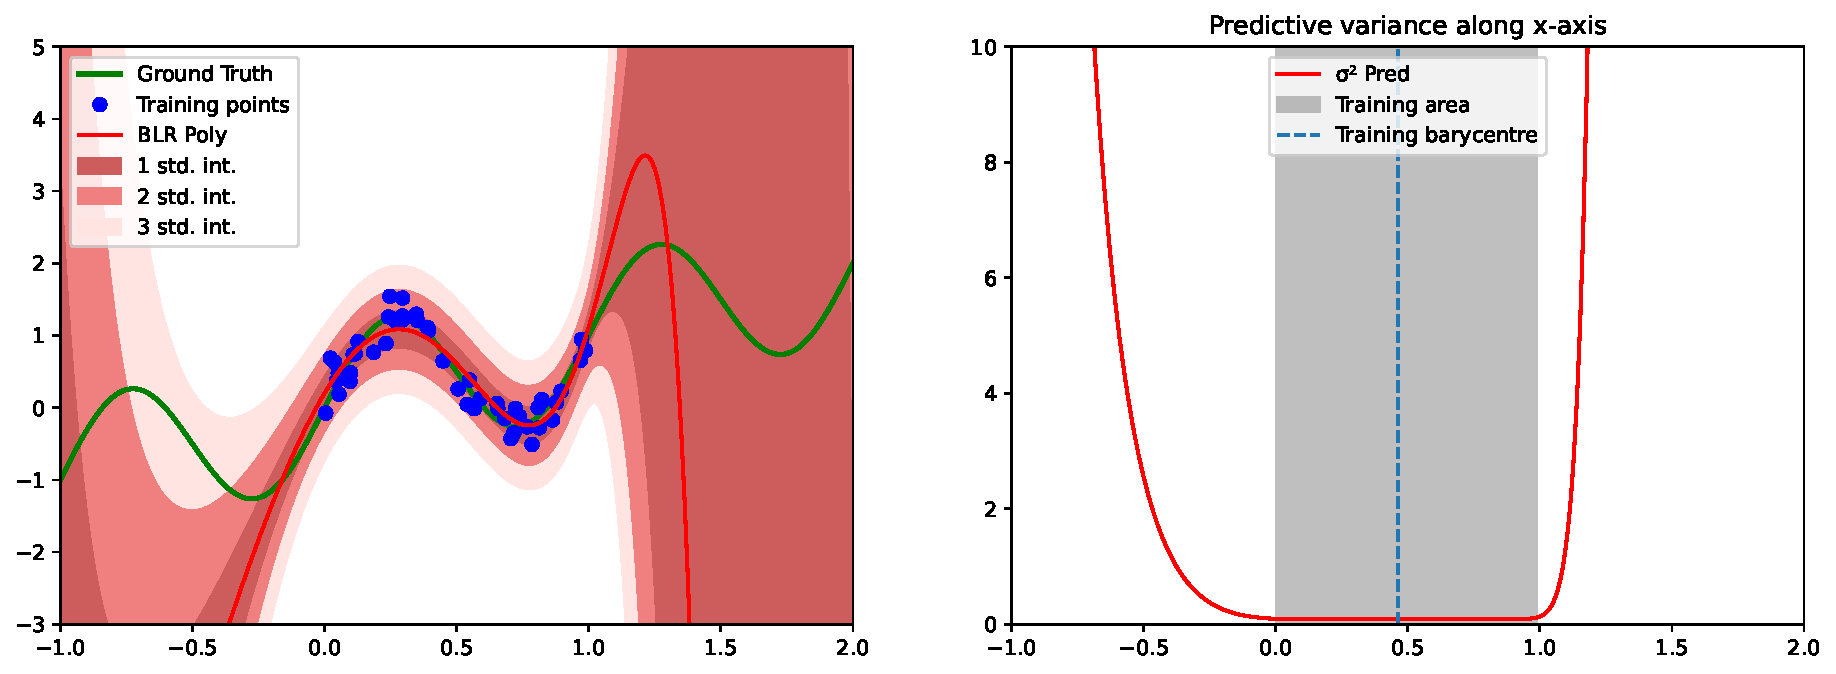
\includegraphics[width=0.95\textwidth]{phi_polynomial.pdf}
    \caption{<caption>}
    \label{fig:phi_polynomial}
\end{figure}

\subsection{Gaussian basis functions}

\paragraph*{2.4. Code and visualize results on sinusoidal dataset using Gaussian basis functions. What can you say this time about the predictive variance?}

...

\begin{figure}[H]
    \centering
    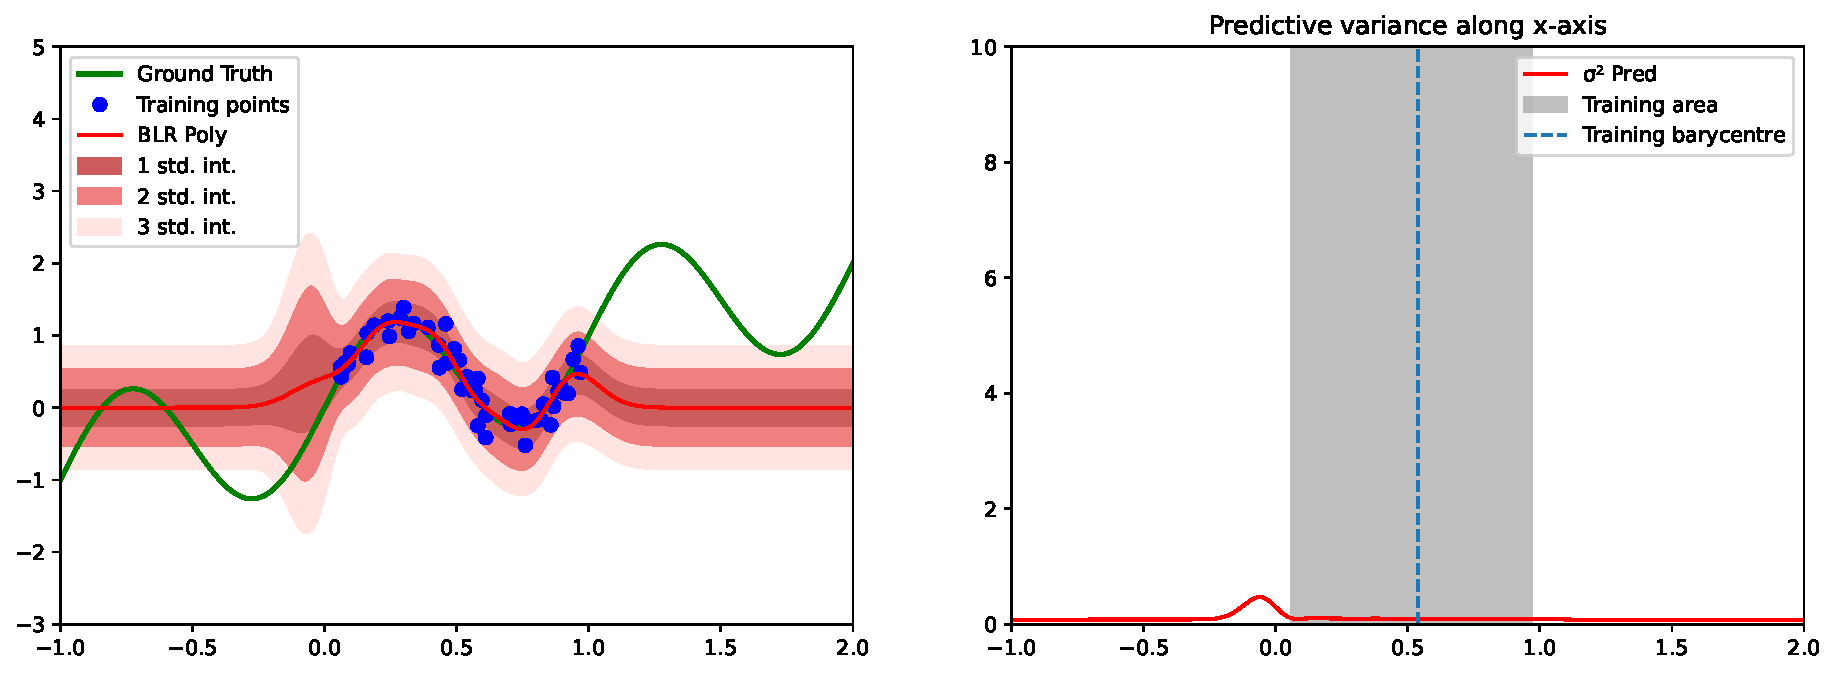
\includegraphics[width=0.95\textwidth]{phi_gaussian.pdf}
    \caption{<caption>}
    \label{fig:phi_gaussian}
\end{figure}

\paragraph*{2.5. Explain why in regions far from training distribution, the predictive variance converges to this value when using localized basis functions such as Gaussians.}


